\section{Characterize {\kvcache} Workload in the Wild}
\label{sec:analyze}

\iffalse
\noindent
We analyze the {\kvcache} usage patterns across requests processed 
by the {\company}'s serving system, 
with particular focus on their temporal and spatial locality,
and why these workloads have such localities. 
\fi

\subsection{Trace data collection}
\label{sec:workload-data}

\begin{figure}[!t]
%        \vspace{2.5mm}
        \begin{minipage}{1\linewidth}
        \hspace{-1mm}        
        \centering    
        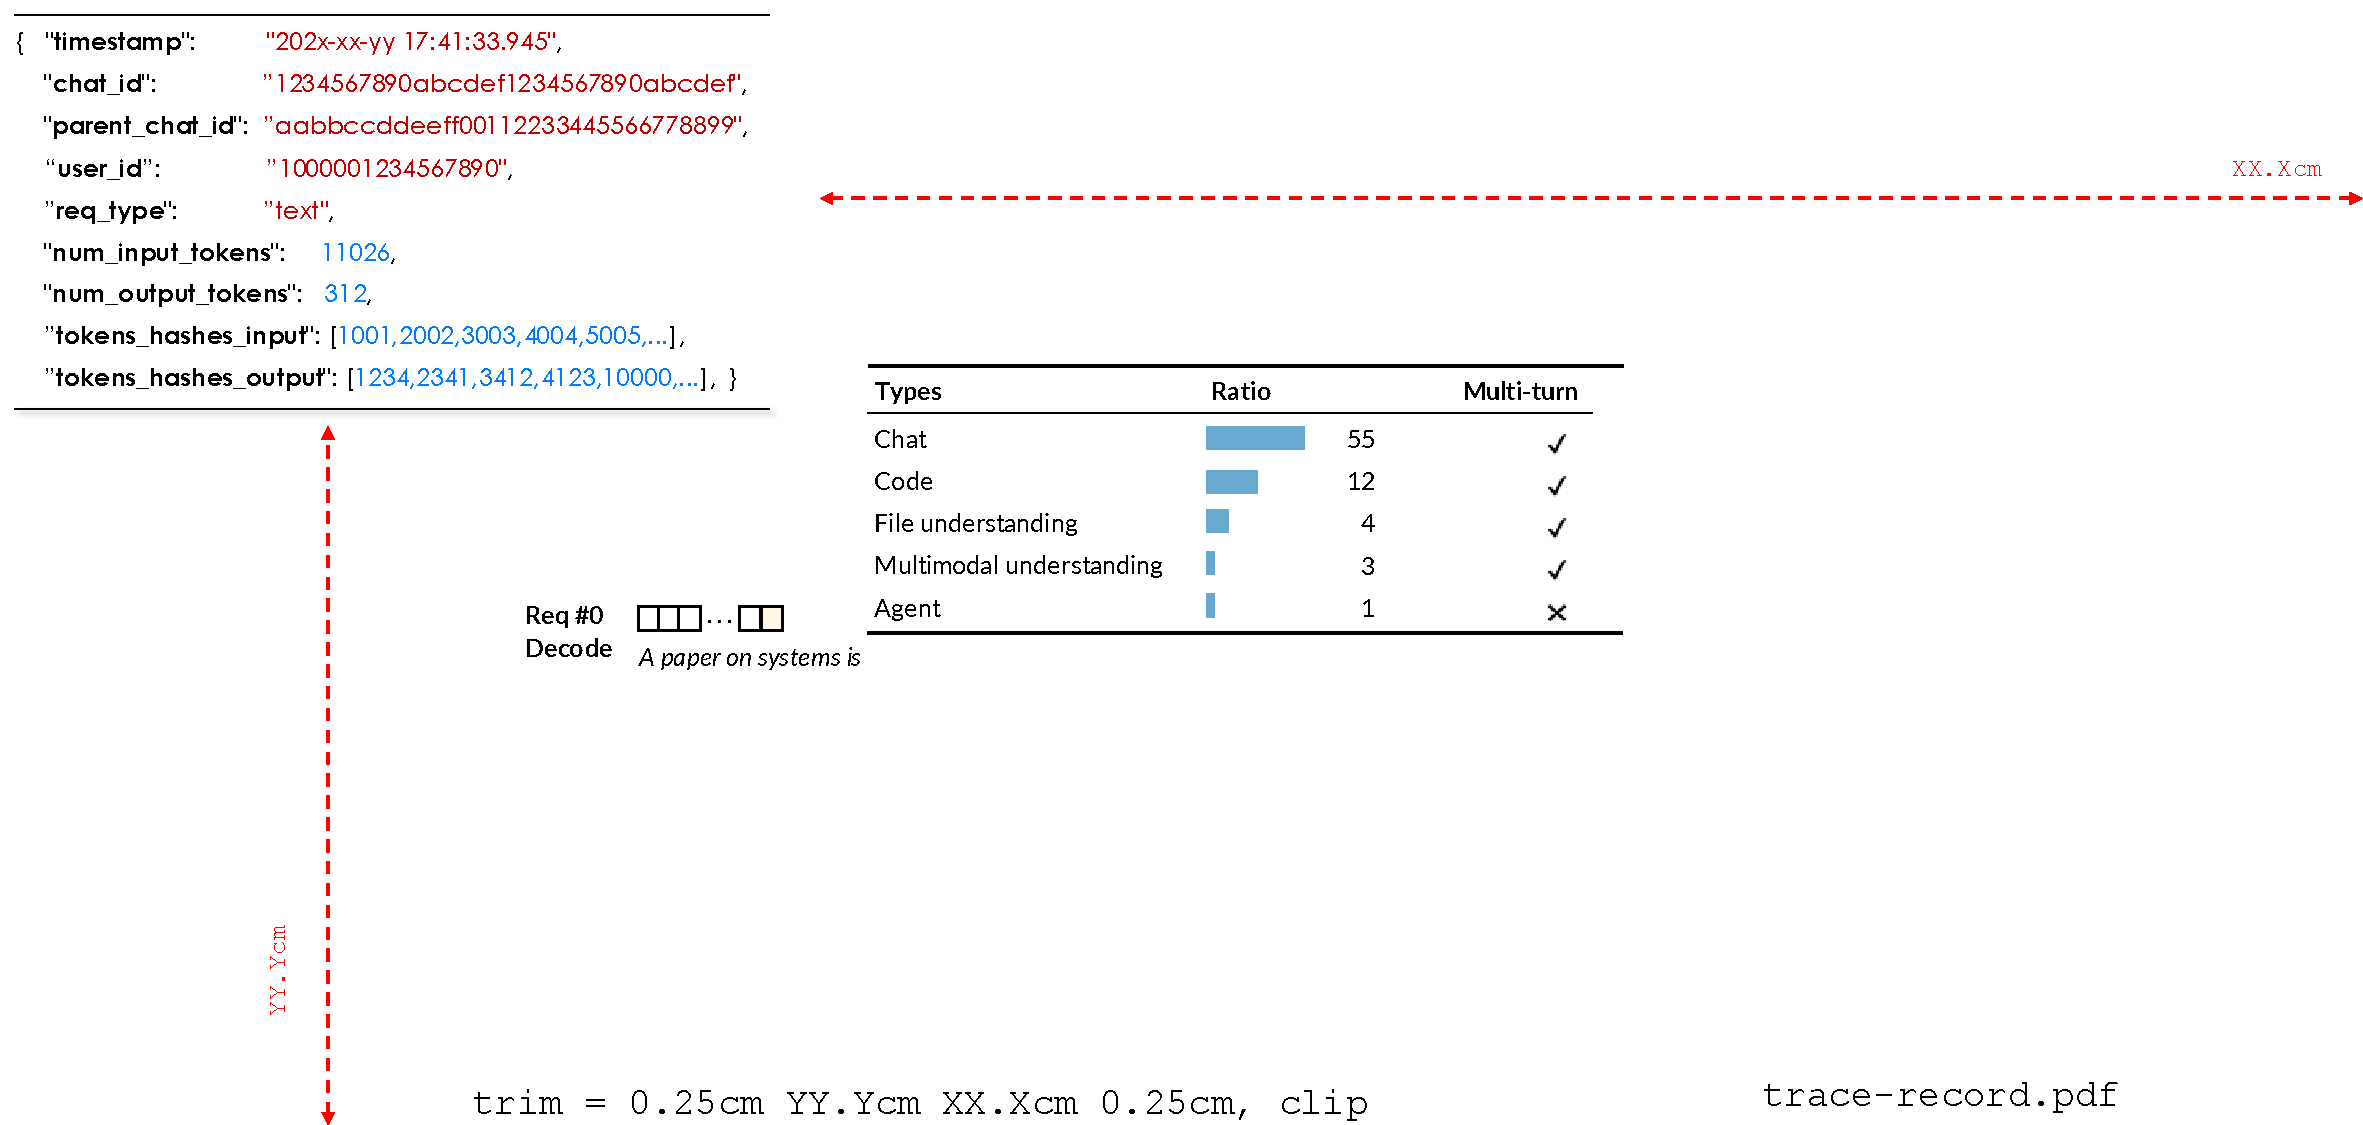
\includegraphics[width=\columnwidth, trim=0.25cm 11.9cm 26.6cm 0.25cm, clip]{figs/trace-record.pdf} 
        \end{minipage} \\[5pt]
        \begin{minipage}{1\linewidth}
        \caption{\small{\emph{
            An example of the collected trace record. 
            %The \texttt{parent\_chat\_id} can be \texttt{None}. 
            }
        }}
        \label{fig:trace-record}
        \end{minipage} \\[-10pt]
        \end{figure}
        
\noindent
We collected and analyzed two weeks (February 2025 and December 2024)
of LLM serving request traces from
one of {\companyfull}'s serving clusters.
For brevity, we present results from one representative day per trace.
The results remain consistent throughout the workdays in each week (see \textsection{\ref{analysis:reuse-evolution}}).
%We have also cross-validated other days and confirmed that the trends are similar.
\emph{Note that we cannot collect the raw input and output for each request
due to {\company}'s strict privacy policy.}
For a specific trace, all its collected requests are served by the same model.

Below, we first describe the detailed anonymized trace record provided by the operational team
of the serving cluster,
then we move on to highlight the differences between two traces,
both representing typical serving workloads nowadays.
{\fig{fig:trace-record}} presents the layout of a collected request:

%\vspace{-1.ex}
\stitle{1. Timestamp: } The time 
when the serving cluster receives the request.  

\stitle{2. Chat ID: } The unique ID of the request. 

\stitle{3. Parent Chat ID (under multi-turn serving): } 
For requests in a multi-turn session,
the serving system assigns a parent ID to each request, linking it to the previous request in the session.
By traversing the parent IDs, we can identify all requests belonging to the same session. 
If the parent ID is empty, then the request is the first-turn of a session
and we call them \emph{single-turn request}. 
Otherwise, we call requests with a non-empty parent ID \emph{multi-turn request}. 

\stitle{4. User ID: }
The unique ID of the user submitting the request. 
These IDs are mapped to a randomly selected domain for anonymity. 

\stitle{5. Request type: } 
The serving gateway categorizes LLM requests into five types:
\emph{Text}: Plain text input via interfaces like ChatBot.
\emph{File}: file analysis (e.g., summarizing document content using LLM).
\emph{Multimodal}: Image understanding through OCR-enhanced processing.
\emph{Search}: Frontend with web-search integrated for knowledge augmentation.
\emph{API}: Programmatic access via OpenAI-compatible interfaces~\cite{openaiapi}.

\stitle{6. Number of Input/Output Tokens: }
The number of input tokens provided to the LLM
and the number of output tokens generated by it.

\stitle{7. The hashed values of In/Output tokens: }
Due to the strict privacy policy,
the runtime system generate the traces 
through salted hashing and domain remapping.
% Specifically, the collector employs default hash~\cite{PEP-456} function
% to generate unique hashes for every four consecutive tokens,
Specifically, the collector employs SipHash~\cite{SipHash} to
generate unique hashes for every four consecutive tokens with random salts per trace,
then remapping the hash IDs to consecutive natural numbers.
This fine-grained hashing enables more fine-grained cache analysis
while enhancing privacy protection compared to single-token hashing.

\stitle{Trace A vs. Trace B. \,}
We collected two traces (A and B) representing two representative LLM serving workloads.
Trace A represents a common to-C (customer) scenario where users interact
with the model through services built by the cloud,
i.e., ChatBot (Text) or File/Multimodal/Search services.
A key feature of to-C workloads is that they are typically human-in-the-loop.
Trace B represents a to-B (business) workload
where business users interact with the LLM by calling OpenAI-compatible APIs hosted by the cloud
through computer programs~\cite{openaiapi}.
API calling is critical for business users because they can systematically leverage
LLM to automate tasks like document translation or user request classification.
Trace B has no request type information because,
similar to the LLM interface calls currently offered by other vendors~\cite{openaiapi,genimiapi,claudeapi},
this information is concatenated on the client side.
%We capture the sequence of tokens obtained by the model after the tokenizer.

\subsection{{\kvcache} reuses analysis in the wild}
\label{sec:workload-patterns}
            
\begin{figure}[!t]
    %\hspace{-3mm}
    \centering
    \includegraphics[width=1.01\linewidth,center]{./data/motiv-cache-hit\figsuffix} \\[2pt]
    \begin{minipage}{1\linewidth}
    \caption{\small{\emph{
        An analysis of 
        the ideal cache hit ratio of the {\kvcache} cache under real-world LLM serving workloads
        within a day. 
        The reported accessed and hit block numbers are normalized (norm.). 
    }}}
    \label{fig:motiv-cache-hit}
    \end{minipage} \\[-0pt]
\end{figure} 

\nospacestitle{How many {\kvcache} can be reused? \,} 
{\fig{fig:motiv-cache-hit}} shows the ideal cache hit rates
on two traces, i.e., assuming a cache having infinite capacity.
We can see that LLM workloads can benefit from caching---it has 62\% and 54\% hit rates
on Trace A and B, respectively.
The hit rate is calculated as follows:
for a total of $N$ {\kvcache} blocks that needed to be computed by LLM in a trace,
if the hit rate is 62\%, this implies that
62\% of the $N$ blocks can reuse a {\kvcache} computed and cached in a prior request.
While the ideal hit ratio is high,
it is smaller than the reported hit ratio
(e.g., more than 80\%~\cite{DBLP:journals/corr/abs-2403-14401,sglang,cachedattention})
on synthetic workloads.
%We calculated the ideal hit rates with a simulator simulating an infinite-capacity {\kvcache} cache. 
\iffalse
The hits are measured based on hashed token blocks, 
where each block contains the KV of four consecutive tokens 
due to the restriction of the collected trace. 
Nevertheless, this granularity is significantly finer than production serving systems; 
for example, vLLM~\cite{vllm} by default uses 16 tokes as its minimal cache block. 
\fi

\begin{figure}[!t]
    %    \vspace{2mm}
        \begin{minipage}{1\linewidth}
        \hspace{-1mm}
        \centering    
        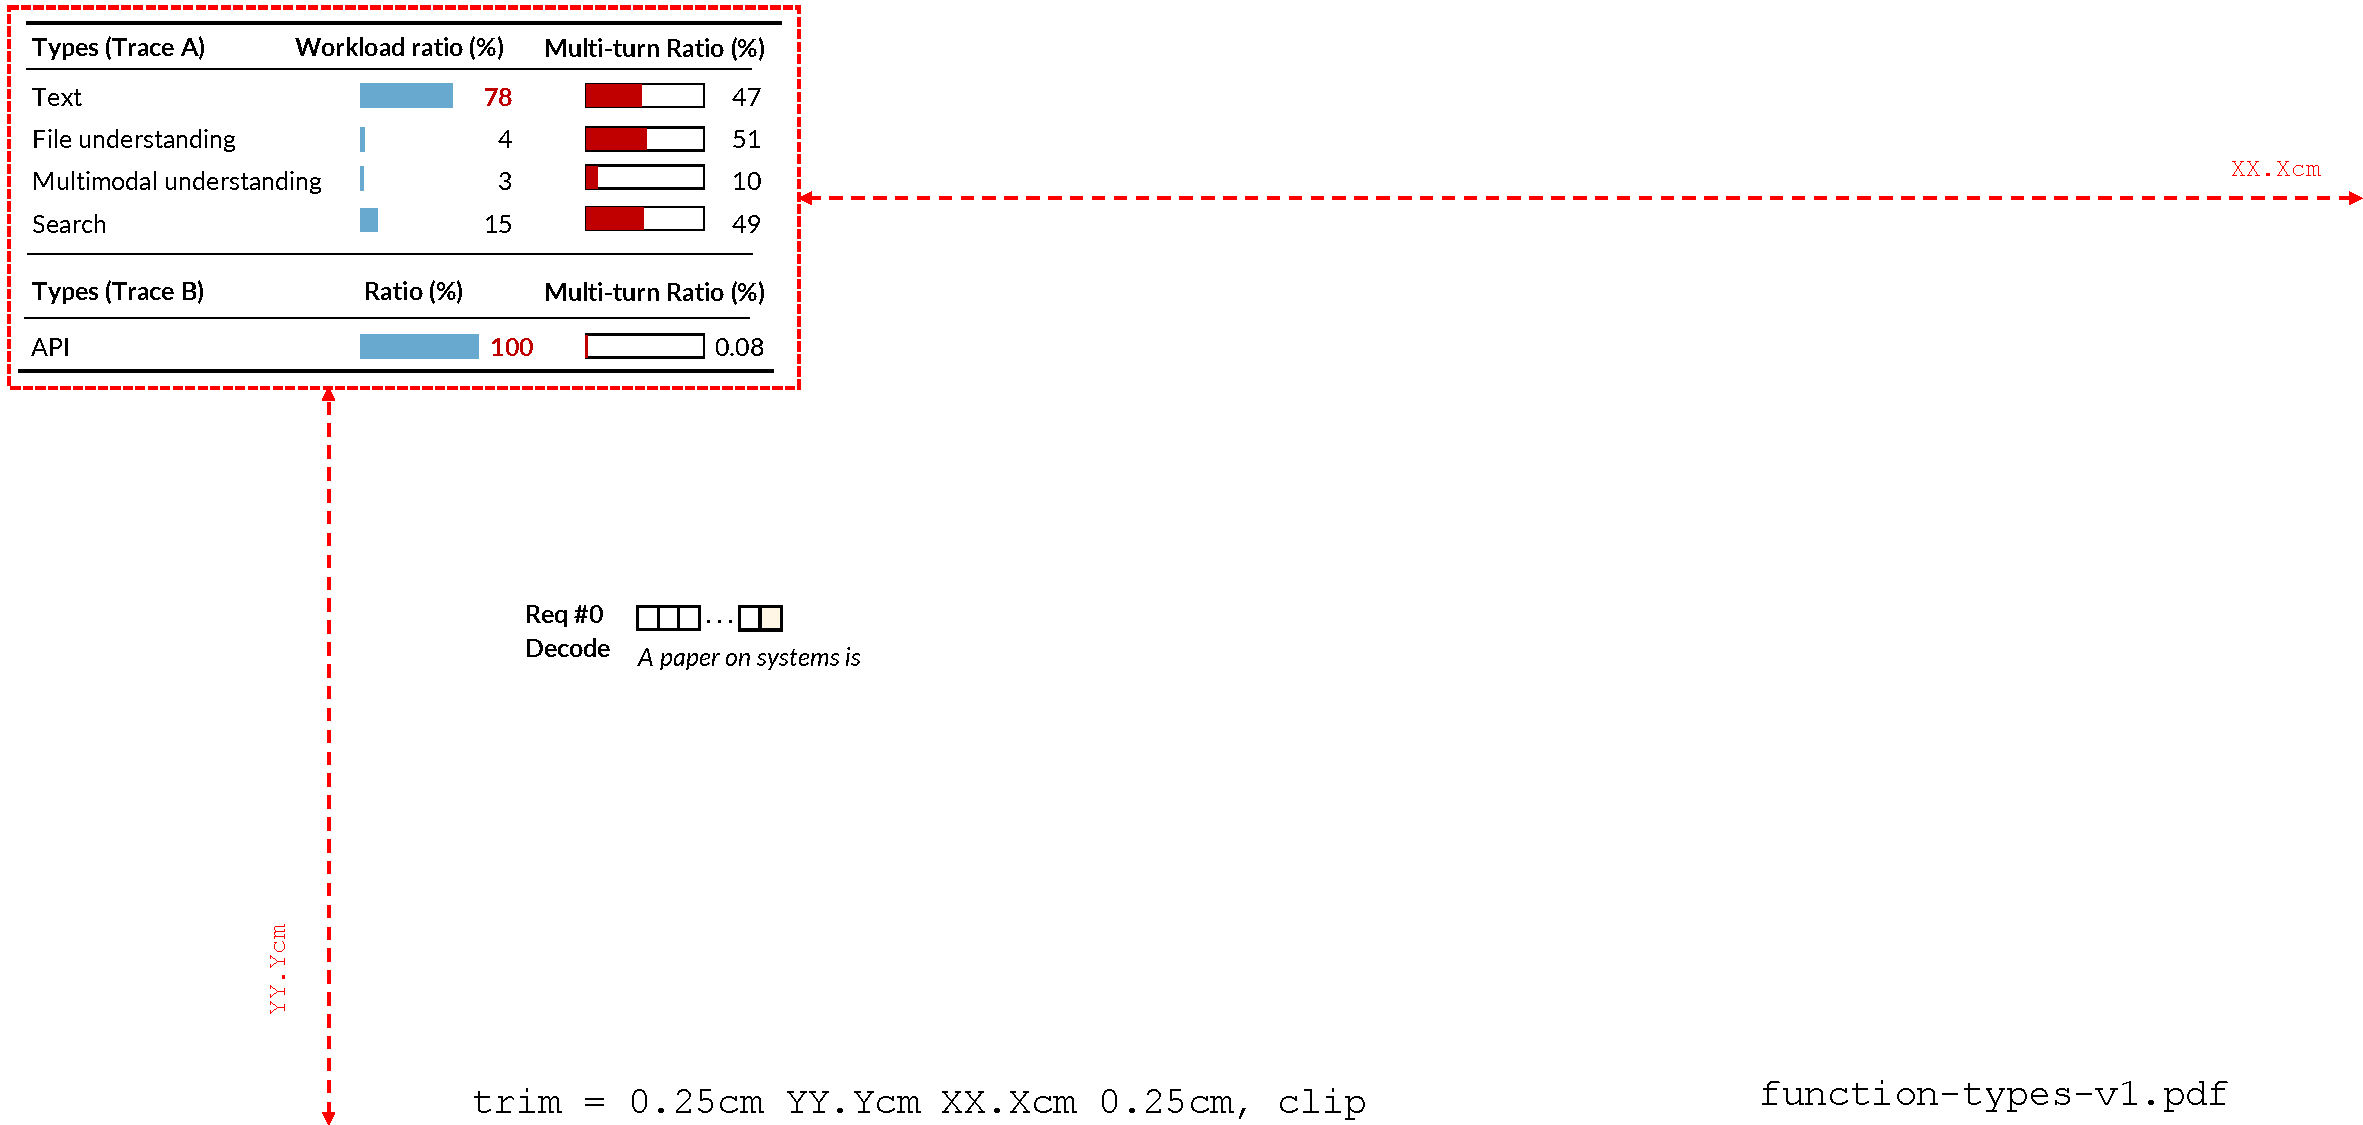
\includegraphics[width=.96\columnwidth, trim=0.25cm 12.54cm 26.9cm 0.25cm, clip]{figs/function-types-v2.pdf} \\[1pt]
        \end{minipage} \\[5pt]
        \begin{minipage}{1\linewidth} 
        \caption{\small{\emph{%
            Workload types and multi-turn ratio of requests in our collected traces. 
        }}}
        \label{fig:motiv-workload-type}
        \end{minipage} \\[-10pt]
        \end{figure}  
  
\stitle{Single-turn and multi-turn requests are equally important for {\kvcache} reuse. \,}        
While it is a common belief that multi-turn requests are key contributors to the cache hits~\cite{DBLP:journals/corr/abs-2403-14401,cachedattention}, 
this is not the case on the to-B workloads (Trace B). 
{\fig{fig:motiv-workload-type}} shows 
the contribution of each request type as well as their multi-turn ratio.
For Trace A, it is dominated by the requests sent by the chatbot (78\,\%),
and all request types except for the multimodal have a similar multi-turn ratio (47--51\,\%).
For Trace B, it only has API requests
with a negligible multi-turn ratio (less than 0.1\,\%).
Nevertheless, the single-turn requests contribute 97\,\% of the total cache hits for Trace B.
% (see {\fig{fig:motiv-cache-hit}}).

Single-turn API requests dominate the hits in to-B workloads for two reasons. 
First, LLM API requests share {\kvcache} through common system prompts. 
Specifically, each request comprises:
(1) a system prompt providing task instructions (e.g., document translation guidelines) and 
(2) a user prompt containing request-specific data (e.g., target document). 
When programs make API calls~\cite{DBLP:conf/osdi/LinHZ00CQ24}, 
they typically hardcode identical system prompts in the program,
thus enabling {\kvcache} sharing across requests, even for single-turn requests.
Second, API requests often exhibit rapid submission rates (e.g., >\,10\,QPS),
enabling frequent reuse of the same shared {\kvcache} from system prompts. 
%This ensures that
%the corresponding {\kvcache} blocks remain persistently retained in cache
%under traditional policies such as LRU.
\iffalse
Second, API requests overwhelm chats in number (see {\fig{fig:motiv-workload-type}}),
and therefore the overall cache hits are much larger. 
We believe this is due to the fact that programs can send requests faster than humans. 
\fi

\begin{figure}[!t]
    %\hspace{-3mm}
    \centering
    \includegraphics[width=1.01\linewidth,center]{./data/cross-hit\figsuffix} \\[-1pt]
    \begin{minipage}{1\linewidth}
    \caption{\small{\emph{
    An analysis of whether a user may hit the {\kvcache} cached by another user.
    The darker the color, the higher the normalized hit count.
    Note that we have amplified the diagonal line in case it is too thin, since
    the trace provider serves numerous users.
    }}}
    \label{fig:motiv-cross-hit}
    \end{minipage} \\[-5pt]
\end{figure} 

\stitle{Cross-user {\kvcache} hits are rare. \,}
{\fig{fig:motiv-cross-hit}} shows the heatmap of the cache hits between users,
assuming an infinite-size {\kvcache} cache.
Darker colors indicate higher normalized hit counts.
We can see that for each user, most hits come from requests submitted
by themselves (the diagonal line).
While users naturally reuse {\kvcache} from their own requests---either
via multi-turn conversations or through programs calling API with
the same system prompt for the same task, the low inter-user hit rate suggests that
users tend to customize their own system prompts rather than
using template prompts provided by third-party libraries~\cite{prompt-library}.
As a result, we suggest paying more attention to intra-user {\kvcache} 
reuses rather than inter-user~\cite{promptcache,sglang,DBLP:journals/corr/abs-2404-12457,DBLP:conf/sigcomm/LiuLCRHZDY0AMHH24}
when designing {\kvcache} systems.

\begin{figure}[!t]
    %\hspace{-3mm}
    \centering
    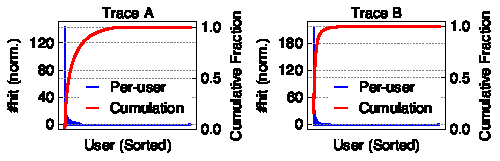
\includegraphics[width=1.0\linewidth,center]{./data/user-hit-distribution.pdf}  \\[1pt]
    \begin{minipage}{1\linewidth}
    \caption{\small{\emph{        
    An analysis of the normalized (norm.) hits contributed by different users
    in an ideal setup with infinite cache size.
    }}}
    \label{fig:motiv-user-hit}
    \end{minipage} \\[-5pt]
\end{figure} 

\begin{figure}[!t]
    %\hspace{-3mm}
    \centering
    \includegraphics[width=1.0\linewidth,center]{./data/user-distribution\figsuffix}  \\[1pt]
    \begin{minipage}{1\linewidth}
    \caption{\small{\emph{        
        An analysis of the normalized (norm.) request count for different users. 
    }}}
    \label{fig:motiv-user-count}
    \end{minipage} \\[-5pt]
\end{figure} 

\stitle{The {\kvcache} reuses are skewed. \,}
{\fig{fig:motiv-user-hit}} shows the {\kvcache} cache hits contributed by different users,
along with the cumulative hits.
The {\kvcache} hit pattern is highly skewed: 19\,\% of the user requests in trace A and 4\,\%
in trace B account for more than 90\,\% of the {\kvcache} block hits.
This skewness stems from two factors.
First, the requests are unevenly distributed across users, especially in Trace B.
{\fig{fig:motiv-user-count}} shows the normalized number of requests sent by different users:
15\,\% of the users (head users) contribute 90\,\% of the requests in Trace B.
Since {\kvcache} hits primarily occur for requests from the same user (see {\fig{fig:motiv-cross-hit}}),
the skewness in request counts is expected to lead to a similar skewness in {\kvcache} hits.
Second, even when requests are sent relatively evenly by different users,
individual users vary significantly in their {\kvcache} hits.
As also shown in {\fig{fig:motiv-user-count}},
Trace A exhibits a moderately skewed request distribution: 19\,\% of users generate 50\,\% of the requests,
and 72\,\% generate 90\,\% of the requests.
Nevertheless,
the {\kvcache} hits are still skewed.
We suspect that this is due to their tendency to engage in multi-turn requests.
\iffalse
Finally, readers may wonder why Trace B has more skewed requests per user than Trace A. 
We suspect that some head business users interact with the LLM more frequently 
with automated tasks. 
\fi

\subsection{Analyses of multi-turn requests features}
\label{sec:motiv-temporal-spatial}

\noindent
We first examine the features of multi-turn requests, as they 
still dominate the {\kvcache} reuse in to-C workloads. 
We omit the results on Trace B because multi-turn requests are rare in it.

\begin{figure}[!t]
    %\hspace{-3mm}
    \centering
    \includegraphics[width=1.0\linewidth,center]{./data/multi-turn-A\figsuffix}  \\[1pt]
    \begin{minipage}{1\linewidth}
    \caption{\small{\emph{        
        Distribution of turn number of multi-turn requests 
        on Trace A. 
    }}}
    \label{fig:motiv-multi-turn-numbersx}
    \end{minipage} \\[-5pt]
\end{figure} 

\stitle{Multi-turn requests have high variability. \,}
We observed two kinds of variability.
First, the number of turns varies significantly across different sessions. 
{\fig{fig:motiv-multi-turn-numbersx}} shows the distributions of turn numbers on Trace A: 
54\,\% of requests are single-turn requests, 
while the 50$^{th}$ and 90$^{th}$ percentile turn numbers are 1 and 5, respectively. 
The distribution has a long tail---the longest session has 232 turns, 
two orders of magnitude larger than the median (232\,$\times$). 


\begin{figure}[!t]
    %\hspace{-3mm}
    \centering
    \includegraphics[width=1.0\linewidth,center]{./data/user-turn-number\figsuffix}  \\[3pt]
%    \includegraphics[width=1.0\linewidth,center]{./data/user-turn-number-deviation-ditribution\figsuffix}  \\[1pt]
    \begin{minipage}{1\linewidth}
    \caption{\small{\emph{        
        An analysis of the mean (upper) 
        and standard deviation (lower) of 
        the number of turns of requests sent by each user. 
        The users are sorted across to their mean number of turn (upper) 
        and standard deviation (lower).
    }}}
    \label{fig:motiv-user-turn-number}
    \end{minipage} \\[-5pt]
\end{figure} 

% Second, as shown in {\fig{fig:motiv-user-turn-number}},
% for each user, the mean turn number is similar to others,
% with only a few outliers that have more turns than the others.
% While the mean has less variance,
% the per-user deviation may vary significantly:
Second, multi-turn request distributions exhibit significant user-level variation.
{\fig{fig:motiv-user-turn-number}} shows that most users have similar mean turn counts,
except for a few head users—the top 10\% exhibit 8.9\,$\times$ more turns than the average.
Additionally, turn count deviations vary substantially, ranging from 1 to 44.
This suggests diverse interaction patterns: some users show high variability, while others remain stable.


\begin{figure}[!t]
    %    \vspace{2mm}
        \begin{minipage}{1\linewidth}
%            \hspace{-1mm}
        \centering    
        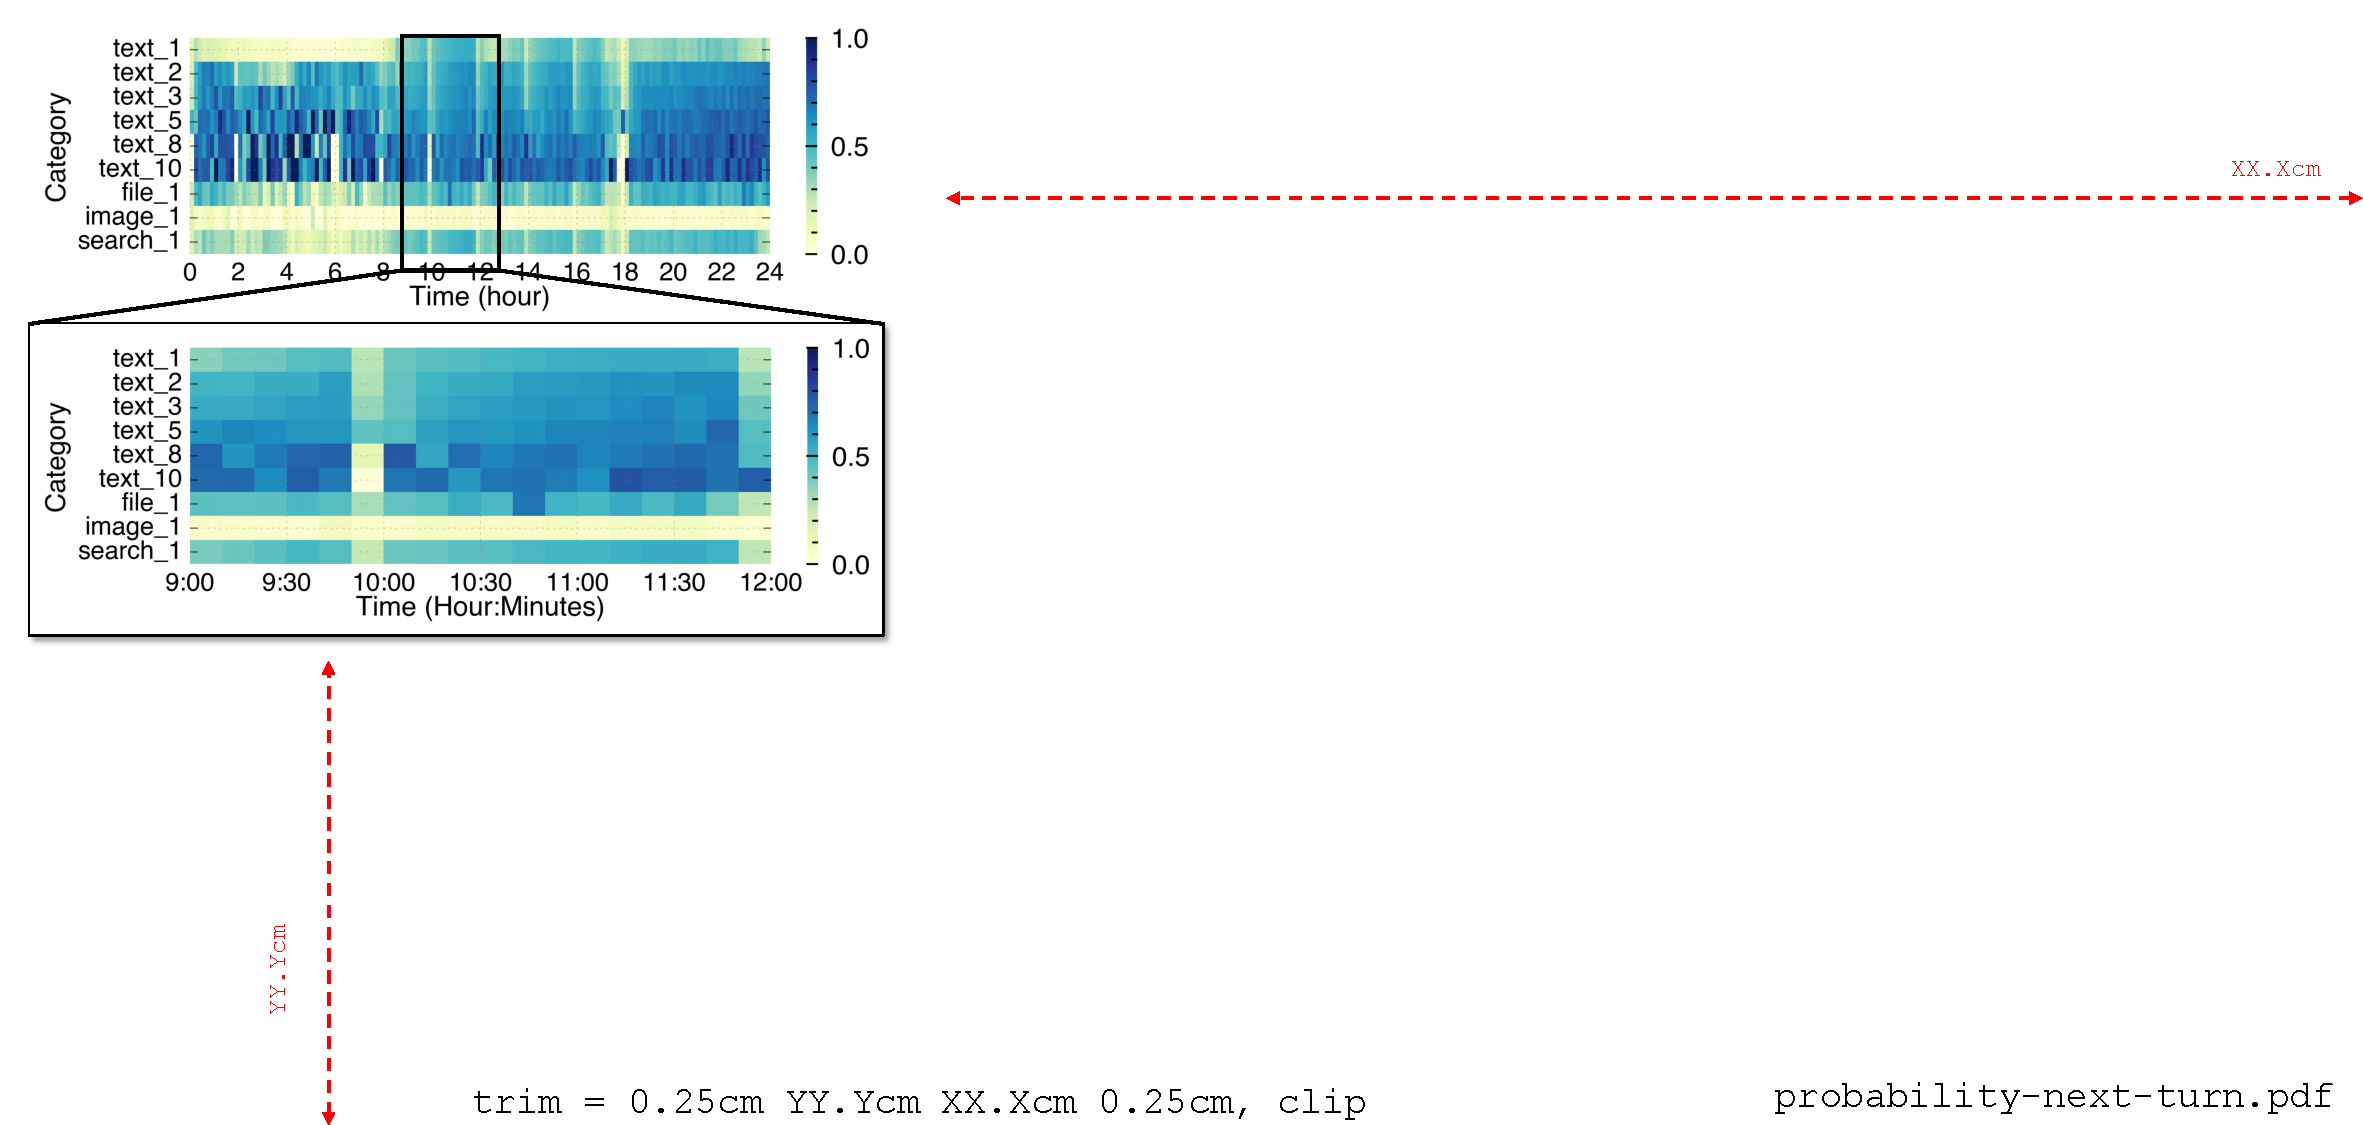
\includegraphics[width=.96\columnwidth, trim=0.25cm 7.9cm 24.1cm 0.25cm, clip]{figs/probability-next-turn.pdf} \\[1pt]
        \end{minipage} \\[5pt]
        \begin{minipage}{1\linewidth} 
        \caption{\small{\emph{%
            An illustration of how the frequencies of issuing the next turn request change over time 
        for different request types.
        The x-axis is the timeline.
        The workload categories are sorted according to their popularity.
        }}}
        \label{fig:motiv-next-turn-probability}
        \end{minipage} \\[-10pt]
        \end{figure}  
  

\stitle{The probability of issuing the next turn request is predictable given a workload category and time interval,
and the probability differs across request categories. \,}
A request category includes both the original request type (e.g., Text and Search)
as well as the turn number of the request,
i.e., a 1-turn text (single-turn text request) is different from the 2-turn text request.
{\fig{fig:motiv-next-turn-probability}} shows a heatmap of how the
probability of issuing the next-turn request changes over the long time interval (24 hours)
as well as a zoomed-in view of a short time interval (3 hours).
The intensity of the color indicates
the profiled frequencies within a time window (10 minutes).
%We categorize the request types by their original type (Text, Search) and current turn,
%e.g., \texttt{text\_1} means a request that is at its first turn.
We can see that though different request categories have different frequencies (shown by vertical lines),
for a specific category,
the frequency of issuing the next-turn request remains consistent over a one-hour time interval
 (shown by horizontal lines).
We attribute this to the fact that the probability distribution of {\kvcache} reuse is quite fixed
given a specific time interval and request category.
\textsection{\ref{sec:motiv-temporal-spatial}} further elaborates on that.
Interestingly, the frequency of issuing the next-turn request differs across request categories.
For example, single-turn requests demonstrate significantly lower rates of 
issuing next-turn requests (mean=0.5) compared to multi-turn requests (mean=0.8).
%The frequency of issuing the next-turn of image requests (Mean<0.1) is relatively lower than other types.
%The frequencies of file and search types are stable (Mean=0.4) over 3-hours time interval.
%\TODO{Refine Descrption}

\subsection{Analyses of temporal and spatial locality}
\label{sec:motiv-temporal-spatial}


\begin{figure}[!t]
    %\hspace{-3mm}
    \centering
    \includegraphics[width=1.0\linewidth,center]{./data/temporal\figsuffix}  \\[-0pt]
    \begin{minipage}{1\linewidth}
    \caption{\small{\emph{      
       The distribution of {\kvcache} reuse time of all requests in Trace A and B. 
    }}}
    \label{fig:motiv-temporal}
    \end{minipage} \\[-5pt]
\end{figure} 

%\noindent
%We now characterize the temporal and spatial locality of {\kvcache}, 
%which are critical for designing caching systems.
\noindent
Temporal locality can be characterized by profiling the distribution of reuse time,
i.e., the interval between when a {\kvcache} block is reused by another request. 

\stitle{{\kvcache} reuse time is short. \,}
{\fig{fig:motiv-temporal}} shows the distributions of {\kvcache} reuse time
on both traces. 
%We align the x-axes of two traces to the same scale
%to better compare the differences.
We can see that the reuse time for both workloads is typically small:
In Trace A, 80\% of the reuse time falls within less than 10 minutes,
while in Trace B it falls within 10 seconds.
The differences lie in the human-in-the-loop versus computer-in-the-loop interactions
that generated the requests in two traces.



\begin{figure}[!t]
    %\hspace{-3mm}
    \centering
    \includegraphics[width=1.0\linewidth,center]{./data/temporal-workload\figsuffix}  \\[1pt]
    \begin{minipage}{1\linewidth}
    \caption{\small{\emph{        
%        Temporal locality for single-turn requests on both traces.
        The distribution of {\kvcache} reuse time of single-turn 
        requests in Trace A and B. B has one category of request (API).
            }}}
    \label{fig:motiv-temporal-workload}
    \end{minipage} \\[-5pt]
\end{figure} 

\begin{figure}[!t]
    %\hspace{-3mm}
    \centering
    \includegraphics[width=1.0\linewidth,center]{./data/time-between-turn\figsuffix}  \\[0pt]
    \begin{minipage}{1\linewidth}
    \caption{\small{\emph{        
        The distribution of {\kvcache} reuse time of multi-turn 
        requests in Trace A and B. B has one category of request (API).
        }}}
    \label{fig:motiv-time-between-turns}
    \end{minipage} \\[-5pt]
\end{figure} 

\stitle{Different workload types have different temporal locality. \,}
First, single-turn requests have much lower locality in the to-C workloads, 
while to-B workloads are the opposite. 
{\fig{fig:motiv-temporal-workload}} reports 
whether a single request can be reused by another single-turn request on both traces
in the middle sub-figures.
As we can see, less than 30\,\% of the single-turn requests are reusable in Trace A, 
but more than 50\,\% of requests can be reused in Trace B. 

Second, different request types show different temporal locality.
{\fig{fig:motiv-time-between-turns}} shows the reuse time distribution of multi-turn requests
categorized by their request types.
We can see that chat requests (Text) shows longer reuse time than 
image understanding (Multimodal), but shorter than file understanding (File).
This stems from workload characteristics:
users typically spend more time processing complex LLM outputs based on file content
than casual outputs from conversational chats.
Conversely, visual information processing occurs faster than textual processing~\cite{rock2010your},
leading to shorter reuse times for image tasks.
Finally, Search workloads exhibit the second-longest reuse time,
as users often require substantial time to analyze the searched results.

\begin{figure*}[!t]
    %\hspace{-3mm}
    \centering
    \includegraphics[width=1.01\linewidth,center]{./data/reuse-time-probability-distribution-hist-new\figsuffix}  \\ [6pt]
    \begin{minipage}{1\linewidth}
    \caption{\small{\emph{       
    An empirical analysis of the reuse time probability distribution of {\kvcache} blocks.
    The columns present data from different request categories.
    The first row: distributions under heavy traffic (daytime).
    The second row: distributions under low traffic (nighttime).
    The third row: a comparison of distributions under different days but with similar traffic patterns.
    }}}
    \label{fig:motiv-reuse-time-probability-hist}
    \end{minipage} \\[-5pt]
\end{figure*} 

\stitle{Given a time period and request category, 
the probability distribution of {\kvcache} reuse time follows an exponential distribution. \,}
\label{analysis:block-reuse-probability}
%While different request categories exhibit diverse reuse time distributions,
%we find that the block reuse probability for a specific category is predictable.
{\fig{fig:motiv-reuse-time-probability-hist}} presents the reuse time probability distribution of {\kvcache} blocks across different request categories. 
For each category, we measure the likelihood of its {\kvcache} reuse at specific time intervals after caching. 
We plot these distributions by counting reuse event frequencies at each second following request execution.

From the results, we draw three key observations. 
First, exponential distributions fit well with the reuse probability given
a request category. 
Second, the probability is workload-aware,
i.e., the distributions of different request categories,
including the same request type but different turns,
are different (e.g., text-1 vs. text-2). This implies a workload-aware design that distinguishes different request categories.
Finally, the distributions of requests with similar traffic patterns
are similar. Take text-1 as an example: as shown in the first row,
the distribution drawn from 9:00--10:00 a.m. is similar to that drawn from 10:00--11:00 a.m.,
but is significantly different from that drawn from the nighttime---3:00--4:00 a.m. (second row).
The distributions are also similar across different days (first row vs. third row).
The first and third observation in combine imply that we can acquire the distribution of a request category
using recent historical data.


\iffalse
We categorize three time periods of a workday according to users' activity frequency:
a peak period (9:00 a.m. to 11:00 a.m.), a low-traffic period
(3:00 a.m. to 5:00 a.m.), and a transition period
(12:00 p.m. to 1:00 p.m., 11:00 p.m. to 12:00 a.m. (midnight)).
We observed that for text_1 type, the reuse probability exhibits a peak between 30 to 60 seconds, 
indicating these blocks would be reused in subsequent 
conversations within this timeframe - a phenomenon consistent with typical user behavior patterns.
{\fig{fig:motiv-reuse-time-probability-multiline}} shows the survival
function for different request categories in future time window during a typical workday,
which is the integral image of {\fig{fig:motiv-reuse-time-probability-hist}}.
As in the previous section, we treat the 1-turn and 2-turn requests as distinct request categories. 
The data points $(x, y)$ in the figure represent: the reuse probability $y$ for this category  
in the subsequent time window $[x, \infty)$ satisfies $P_{\text{reuse}}(t \geq x) = y$. 
While different categories exhibit varying reuse time scales (x-axis dimensions),  
they all conform to a long-tailed distribution.
First, the reuse probability of {\kvcache} blocks  
remains high within a brief temporal window (seconds-level), subsequently decays rapidly,  
and stabilizes at a residual level over prolonged periods.  
Second, during peak periods, probability distributions demonstrate cross-time-range
consistency, whereas low-traffic periods show divergence.
We attribute this to the collective user behavior exhibits higher predictability
than individual user patterns.
Therefore, we can predict the next hour's reuse probability distribution with time
based on current hour in the peak time.
Consequently, a {\kvcache} cache system can leverage this feature, 
combined with the predictability of reuse frequencies (see {\fig{fig:motiv-next-turn-probability}})
to improve the cache eviction policy. 
Consequently, during peak periods, we can predict hourly reuse probability distributions  
$\hat{P}_{t+1}$ using current-hour observations $P_t$.
\fi

\begin{figure}[!t]
    %\hspace{-3mm}
    \centering
    \includegraphics[width=1.0\linewidth,center]{./data/spatial-v1\figsuffix}  \\[-3pt]
    \begin{minipage}{1\linewidth}
    \caption{\small{\emph{        
      Overall spatial locality of two traces.
    }}}
    \label{fig:motiv-spatial}
    \end{minipage} \\[-5pt]
\end{figure} 

\begin{figure}[!t]
    %\hspace{-3mm}
    \centering
    \includegraphics[width=1.0\linewidth,center]{./data/spatial-multi-traceC\figsuffix}  \\[-5pt]
    \begin{minipage}{1\linewidth}
    \caption{\small{\emph{        
        The spatial locality of multi-turn requests on Trace A.
    }}}
    \label{fig:motiv-spatial-multi}
    \end{minipage} \\[-5pt]
\end{figure} 


\stitle{Spatial locality. }
{\fig{fig:motiv-spatial}} shows the overall spatial locality of {\kvcache} across both traces.
%Meanwhile, {\fig{fig:motiv-spatial-workload}} and \fig{fig:motiv-spatial-multi}
%further report the locality for single-turn and multi-turn requests, respectively.
We characterize the spatial locality by measuring the ideal cache hit ratio
with various cache strides, i.e., the percentage of tokens cached per request,
as well as different starting token offsets for caching.
This gives a two-dimensional heatmap,
for example, offset (10\,\%, 10\,\%) means that for each request,
we only cache 10\,\% of the tokens starting from the 10\,\% token position.

First, {\kvcache} shows better spatial locality when caching from the beginning,
which is expected since only requests with identical prefixes can share the {\kvcache} (\textsection{\ref{sec:bg}}).
We emphasize this seemingly trivial point because some {\kvcache} optimizations~\cite{DBLP:journals/corr/abs-2410-03065} cache
the tail tokens of requests to hide {\kvcache} load time through concurrent computation and loading.
However, this approach may reduce spatial locality,
as {\fig{fig:motiv-spatial-multi}} particularly demonstrates that reusing intermediate parts
in the cache yields minimal benefits for multi-turn conversations.


\begin{figure*}[!t]
    %\hspace{-3mm}
    \centering
    \includegraphics[width=0.95\linewidth,center]{./data/spatial-workload-cd\figsuffix} \\[-4pt]
    \begin{minipage}{1\linewidth}
    \caption{\small{\emph{
        The spatial locality of single-turn requests. 
    }}}
    \label{fig:motiv-spatial-workload}
    \end{minipage} \\[-5pt]
\end{figure*} 

Second, the spatial locality, like temporal locality, is also workload-aware.
In {\fig{fig:motiv-spatial-workload}}, we observed workloads
like text and multimodal exhibit obvious spatial locality,
while file and search exhibit almost no spatial locality.
Due to the lack of user input content,
we suspect the cause as follows:
the applications add a fixed system prompt for text and multimodal workloads,
whereas the system prompt for file and search is dependent on user inputs.

Finally, we found that increasing the stride size implies a higher cache hit ratio in Trace A ({\fig{fig:motiv-spatial-multi}}),
but it is not the case in Trace B (the last column in {\fig{fig:motiv-spatial-workload}}).
In Trace A, multi-turn requests contribute to the cache hits,
so caching more tokens for a request will lead to more cache hits.
In Trace B, only the system prompt contributes to the cache hits.
Thus, caching a stride of 50\,\% of the request already achieved a peak hit ratio of 50\,\%.
This implies that most system prompt lengths are below 50\% of the total request length in Trace B,
though we don't have the detailed request to support this suspicion.

\subsection{Analyses of {\kvcache} cache capacity requirement}
\label{sec:analyze-capacity}

\noindent
Determining the right cache capacity is critical for a caching system.
Unlike traditional storage systems,
the cached {\kvcache} is ephemeral, so identifying the right size requirement
can save platform costs.
This section analyzes the {\kvcache} capacity using a bottom-up approach:
First, we characterize the features of the lifespan of requests' {\kvcache}.
Then we analyze the storage usage of each request.
In combination, this gives us an estimation of the total {\kvcache} capacity required. 


% \begin{figure}[!t]
%     %    \vspace{2mm}
%         \begin{minipage}{1\linewidth}
% %            \hspace{-1mm}
%         \centering    
%         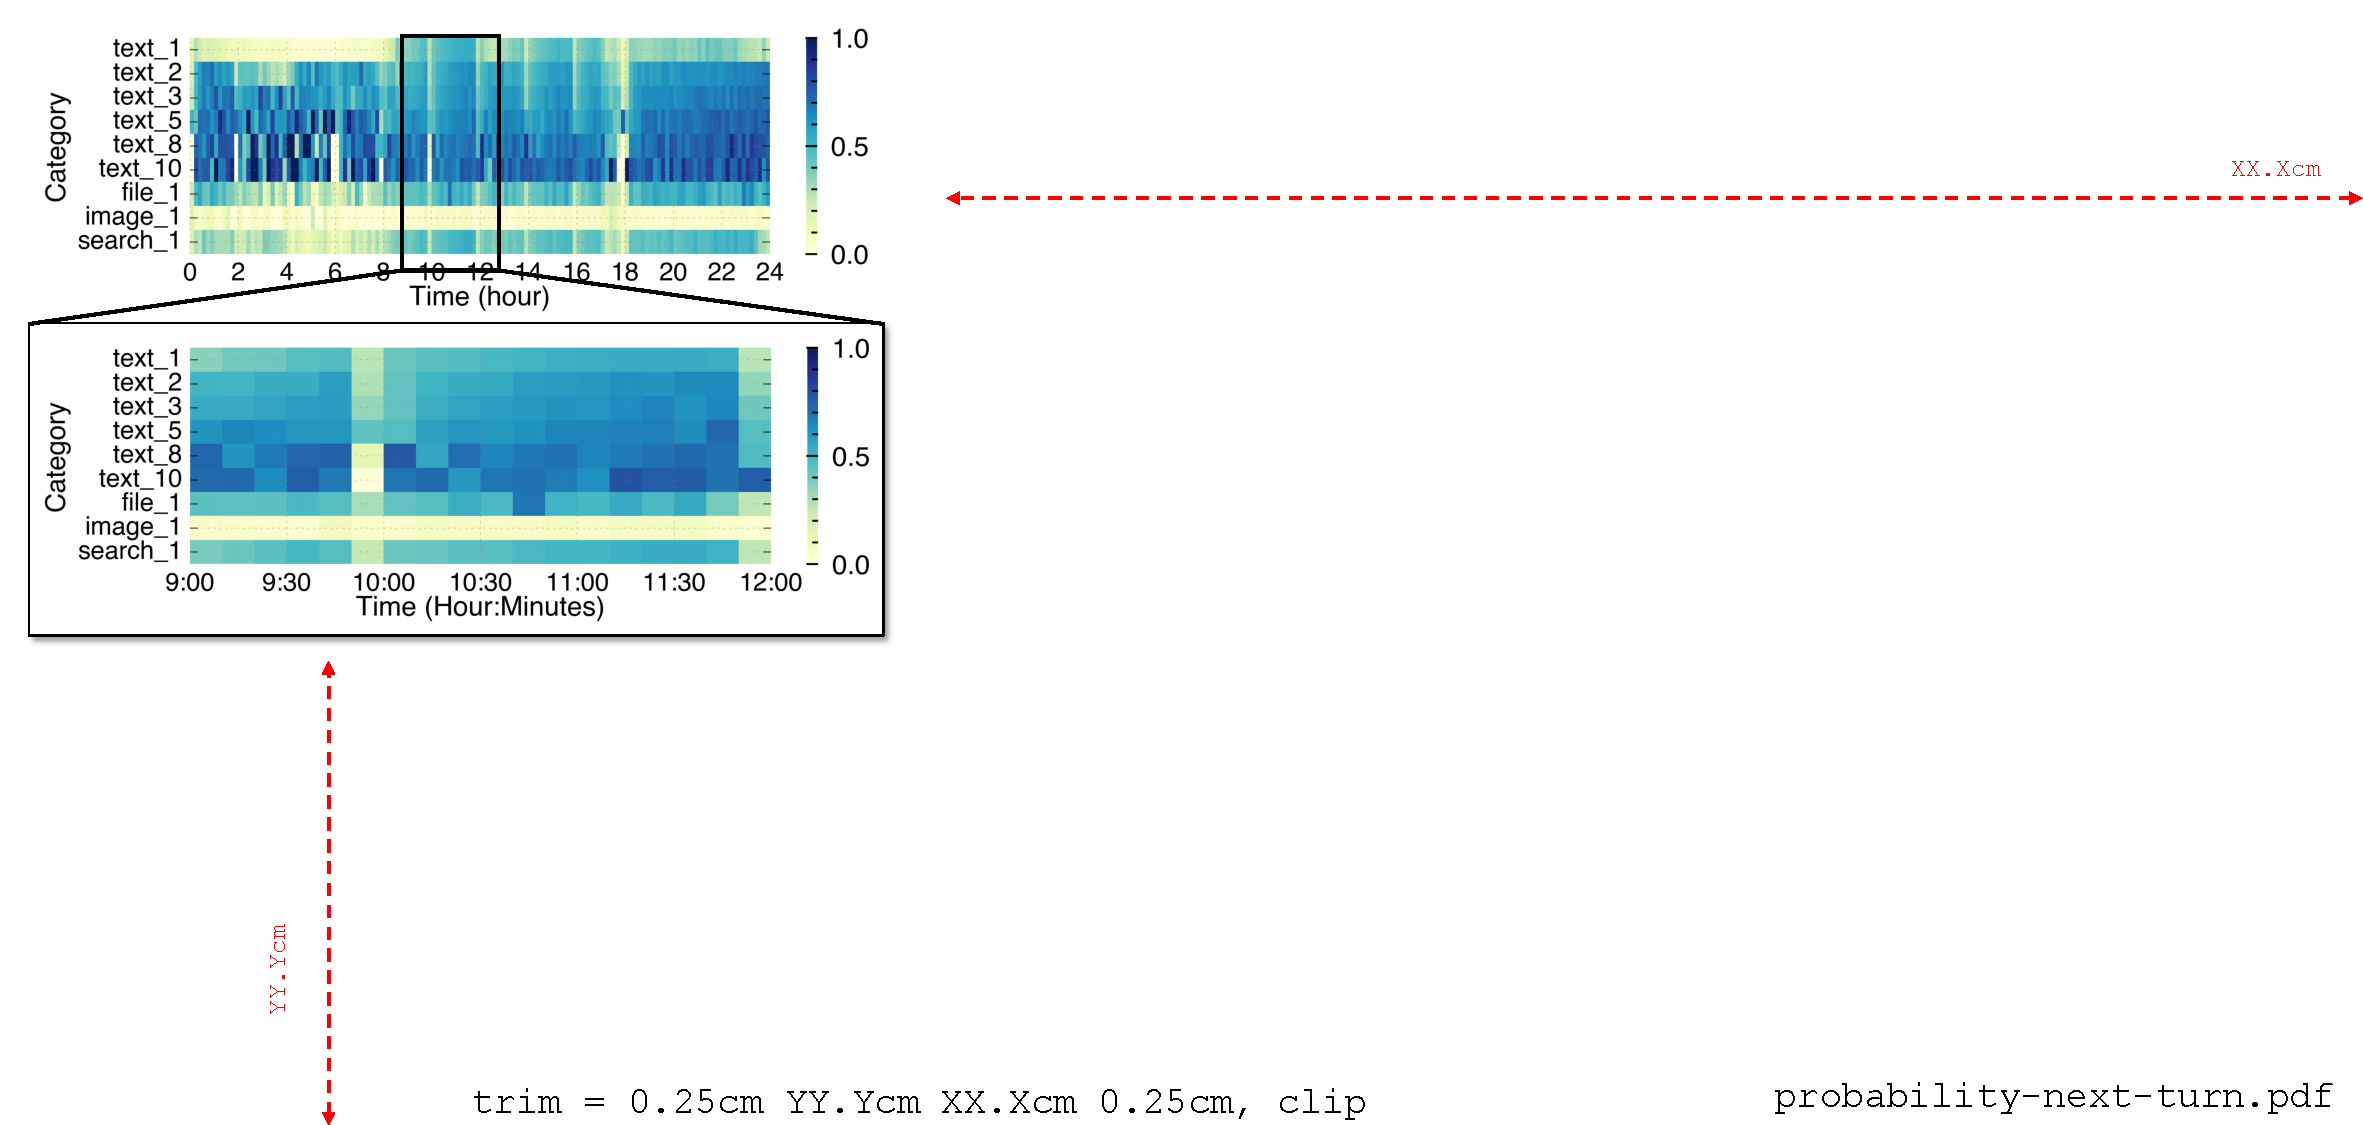
\includegraphics[width=.96\columnwidth, trim=0.25cm 7.9cm 24.1cm 0.25cm, clip]{figs/probability-next-turn.pdf} \\[1pt]
%         \end{minipage} \\[5pt]
%         \begin{minipage}{1\linewidth} 
%         \caption{\small{\emph{%
%             An illustration of how the frequencies of issuing the next turn request change over time 
%         for different request types.
%         The x-axis is the timeline.
%         The workload categories are sorted according to their popularity.
%         }}}
%         \label{fig:motiv-next-turn-probability}
%         \end{minipage} \\[-10pt]
%         \end{figure} 

\begin{figure}[!t]
    %\hspace{-3mm}
    \centering
    \includegraphics[width=1.0\linewidth,center]{./data/block-timespan-cdf\figsuffix}  \\[0pt]
    \begin{minipage}{1\linewidth}
    \caption{\small{\emph{        
        The distribution of the lifespan of {\kvcache} blocks on both traces. 
    }}}
    \label{fig:motiv-block-timespan}
    \end{minipage} \\[-5pt]
\end{figure} 

\stitle{{\kvcache} lifespan is ephemeral and predictable. }
{\fig{fig:motiv-block-timespan}} analyzes the lifespan of {\kvcache} blocks.
A {\kvcache} block ``dies'' if it has not been reused anymore.
We can see that most {\kvcache} blocks ``live'' shortly.
% \TODO{this is paper's version}
% For example, in Trace A, 90\% of the {\kvcache} blocks are not reused after 245 seconds,
% and the number for Trace B is 1.3 seconds.
In Trace A, 90\,\% of the {\kvcache} blocks are not reused after 612 seconds,
and the number for Trace B is 0.3 seconds.
This aligns with our analysis in the previous sections,
e.g., many multi-turn requests will have a short reuse time ({\fig{fig:motiv-temporal}}),
and most requests have a few turns ({\fig{fig:motiv-multi-turn-numbersx}}).
As a multi-turn request ends, its {\kvcache} will not be reused anymore.
Blocks in Trace B have a shorter lifespan despite some outliers.
Unlike Trace A,
most of its cached {\kvcache} blocks are reused for system prompts,
so they can be reused after a long time.
For example, in Trace B, the longest lifespan is 1,200 minutes
while it is 800 minutes in Trace A.
\iffalse
We attribute this overall short lifespan to the extreme skewness in Trace B:
as we have discussed in \textsection{\ref{sec:workload-patterns}},
in Trace B, some head users contribute most of the requests (see {\fig{fig:motiv-user-count}}),
so only a few {\kvcache} will be frequently reused. 
We can see that in {\fig{fig:motiv-block-timespan}}, Trace B has some 
tail {\kvcache} with a long lifespan.
\fi

\begin{figure}[!t]
    %\hspace{-3mm}
    \centering
    %\includegraphics[width=1.0\linewidth,center]{./data/block-timespan-probability-cd\figsuffix}  \\[1pt]
    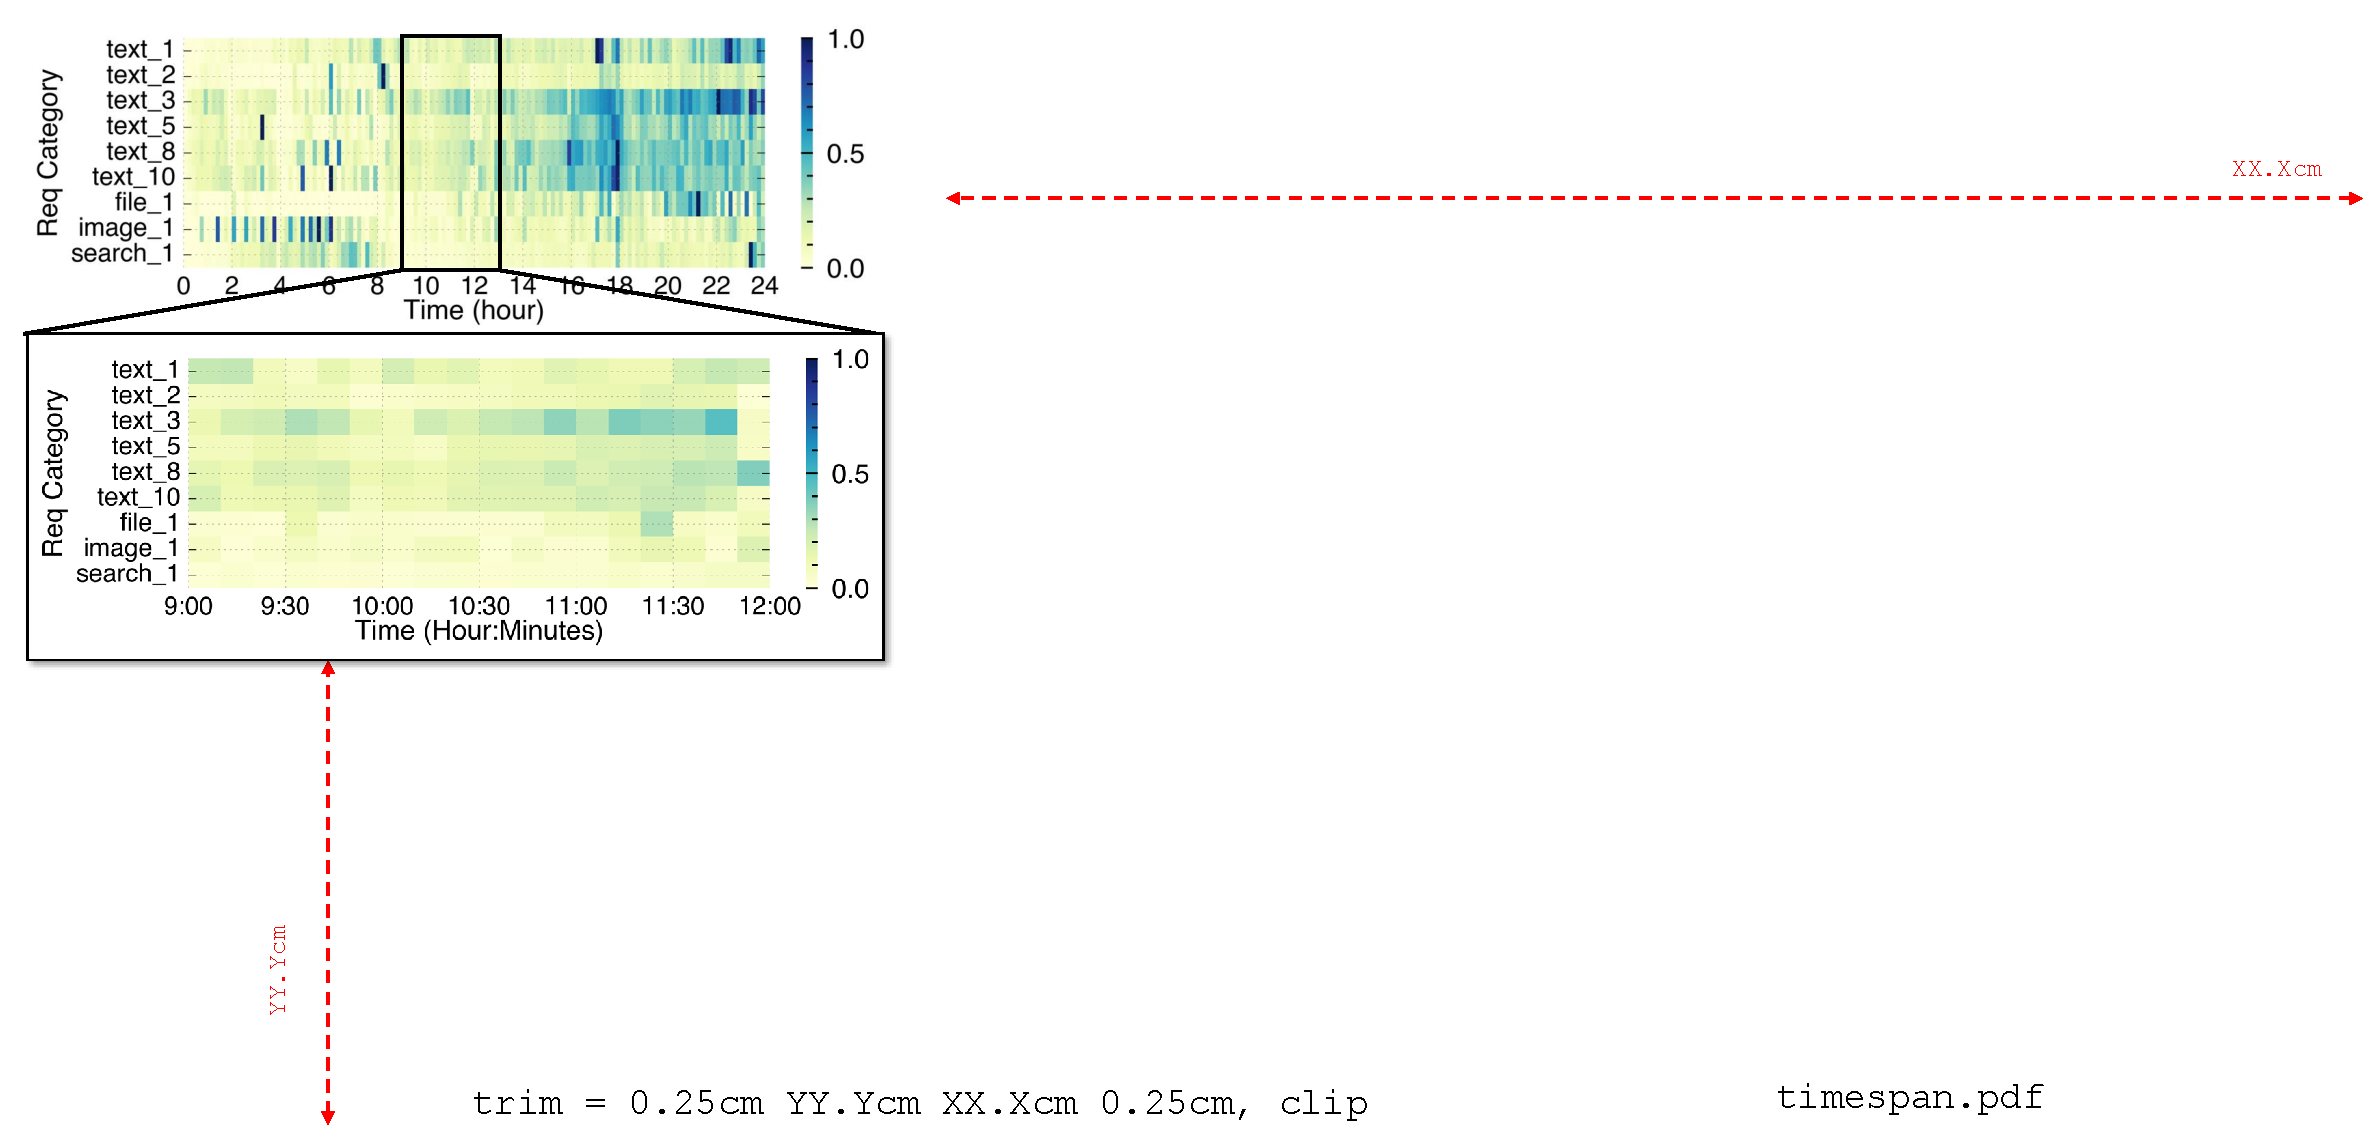
\includegraphics[width=.96\columnwidth, trim=0.25cm 7.85cm 24.1cm 0.25cm, clip]{figs/timespan.pdf} \\[5pt]
    \begin{minipage}{1\linewidth}
    \caption{\small{\emph{        
        An illustration of how the mean lifespan of 
        {\kvcache} blocks changes over time for different request categories. 
        Note that the x-axis represents the timeline.
        The request categories are sorted according to their usage.
    }}}
    \label{fig:motiv-block-timespan-probability}
    \end{minipage} \\[-5pt]
\end{figure} 


%\stitle{{\kvcache} lifespan changes over time. }

{\fig{fig:motiv-block-timespan-probability}} further shows how the mean lifespan of {\kvcache} blocks
changes over time for different request categories.
In the graph, the color intensity represents the normalized lifespan,
with darker colors indicating longer-lived {\kvcache} blocks.
We can see that although the average lifespan at the 24-hour scale is changing over time,
when we zoom in to a smaller timescale (9:00 a.m. to 11:00 a.m.),
the pattern is quite stable.
This implies that we can predict the lifespan of a {\kvcache} block
using historical data to reduce the {\kvcache} cache size
for saving costs,
as storing {\kvcache} at fast storage medium (e.g., CPU's DRAM) is expensive. 

\begin{figure*}[!t]
    %\hspace{-3mm}
    \centering
    \includegraphics[width=1.01\linewidth,center]{./data/size-v2\figsuffix} \\[2pt]
    \begin{minipage}{1\linewidth}
    \caption{\small{\emph{
        The distribution of {\kvcache} size of requests on different traces for \uline{S}ingle 
        and \uline{M}ulti-turn requests. 
        The size is normalized to the 
        GPU memory (HBM) available for serving. 
        The number in the tuple inside each graph represents the length of input and output.
    }}}
    \label{fig:motiv-cache-size}
    \end{minipage} \\[-0pt]
\end{figure*}

\stitle{Per-request {\kvcache} cache usage is moderate. }
A key factor when considering caching is the size of {\kvcache} to be cached,
which is proportional to the input length of each request and
the corresponding model output length.
{\fig{fig:motiv-cache-size}} shows the size distribution of requests on different traces.
Note that we report the relative size when normalized to the HBM available for serving the request
on a serving instance\footnote{\footnotesize{A serving instance
is the minimal number of GPUs required to serve a model.
For example, the serving instance of an 8\,B model only needs one GPU,
while serving a 72\,B model requires 4 in the common case. }}.
This is because a relative value
gives more intuitive results on the capacity required to cache
the {\kvcache} of each request.
The available HBM for {\kvcache} is calculated by subtracting the total HBM of the GPU(s)
in a serving instance from the model parameter and activation sizes.
Since the {\kvcache} size of each request depends on the detailed attention mechanism of the model,
we report the results on three representative models with two widely used attention methods:
group query attention (GQA~\cite{DBLP:conf/emnlp/AinslieLJZLS23}) and multi-head attention (MHA~\cite{DBLP:conf/nips/VaswaniSPUJGKP17}).
GQA uses less memory for the {\kvcache}.

We can see that the overall size of the {\kvcache} is moderate compared to the HBM.
Take Trace A as an example.
On GQA models like Qwen2-7B,
the 50$^{th}$, 90$^{th}$, and 99$^{th}$ HBM usage of the request in Text---the dominant request type
are 0.09\,\%, 0.15\,\%, and 0.37\,\% and 0.36\,\%, 1.31\,\%, and 2.21\,\% for single-turn and multi-turn requests,
respectively.
The average usage is 0.09\,\% and 0.56\,\% for single- and multi-turn requests, respectively.
This small usage is due to the fact that each token consumes few megabytes and
requests in production traces tend to be small:
in Qwen2-7B, it consumes 0.875\,MB {\kvcache} for 16 tokens,
while the mean total token lengths (input+output) for single-turn and multi-turn is 973 and 5,953, respectively.
% while the p50 lengths for single-turn and multi-turn on Trace A are 673 and 5,363, respectively.
For other models, though Llama3-70B also adopts GQA,
it has a slightly higher HBM usage due to the reduced number of GPUs per instance: the
parameter size increases 10\,$\times$ while the number of GPUs we measured only increases 4\,$\times$.
Finally, MHA models have the highest usage due to the increased {\kvcache} per token.
Note that recent open-source models tend to use GQA (or other
attention with even fewer {\kvcache} per token like MLA~\cite{liu2024deepseek}).

Considering that each serving instance typically processes a few requests per second,
our characterization implies that an instance can cache a request for a modest time---e.g.,
for Qwen2-7B, suppose a GPU can process 5 requests per second,
it takes at least 1 minute to saturate the HBM assuming an average 0.32\,\% HBM per request (derived
with a 47\,\% multi-turn ratio of Text request type).
This time is within the reuse distance of {\kvcache} in many scenarios (e.g., API).
Note that in practical setups, we may not achieve such a long reuse time
due to tail requests (e.g., we do observe long context requests with more than 12,000 tokens),
and LLM serving systems typically serve requests in large batches to improve computation utilization.


\begin{figure}[!t]
    %\hspace{-3mm}
    \centering
    \includegraphics[width=1.0\linewidth,center]{./data/opt-cache-space\figsuffix}  \\[3pt]
    \begin{minipage}{1\linewidth}
    \caption{\small{\emph{        
    An analysis of the {\kvcache} cache size required
    to achieve an ideal cache hit ratio on different models and traces.
    The data is collected from 10:00 a.m. to 11:00 a.m.
    }}}
    \label{fig:motiv-opt-cache-space}
    \end{minipage} \\[-5pt]
\end{figure} 

\stitle{Overall memory required for {\kvcache} cache is moderate. }
We analyze the {\kvcache} cache capacity required
by measuring how large a cache can ensure an ideal cache hit ratio
assuming an ideal eviction policy,
i.e., never evict a {\kvcache} that will be reused.
%{\fig{fig:motiv-opt-cache-space}} shows the results.
The measurement is as follows:
at a given time, upon processing a request,
we update the {\kvcache} size by adding the {\kvcache}
of this request if it will be reused,
and subtracting the size of all cached {\kvcache} that will never be reused.
One tricky thing is that
the size required is dependent on the number of serving instances deployed for a workload:
if the instances are over-provisioned, then the estimated requirement would be small.
To obtain the maximal requirement,
we use a setup that uses the minimal number of serving instances,
i.e., each instance serves with the maximum QPS,
so there is no over-provisioning.

{\fig{fig:motiv-opt-cache-space}} shows the results normalized to the
total HBM of a serving instance.
We can see that GQA models require a relatively small cache capacity to reach an ideal cache hit rate:
in Trace A, Llama3-70B only needs 4\,$\times$ of the available HBM for {\kvcache}.
This is typically achievable in modern serving clusters without the need for more storage hierarchies
like remote memory or SSD~\cite{cachedattention}.
For example, in a typical setup featuring 8 A100 GPUs and 1\,TB of CPU memory,
each GPU has access to an average of 128\,GB of CPU memory,
which is nearly 4\,$\times$ the amount of HBM space reserved for storing the {\kvcache}.
Moreover, for Trace B, the {\kvcache} capacity is even smaller than the reserved HBM,
so caching on GPU may be sufficient.

Though GQA needs small cache, 
we should note that MHA models do require a huge amount of {\kvcache} cache,
This is due to their huge per-token KV pairs (see {\fig{fig:motiv-cache-size}}). 
Thus, optimizing cache eviction policies is still important under 
limited cache capacity. 



